% =====================================================================
%  Workload Pressure Analysis — Professional Report
%  Self-contained LaTeX source. Compile with:
%      pdflatex workload_pressure_report.tex
%      pdflatex workload_pressure_report.tex   % second pass for refs
% =====================================================================
\documentclass[11pt,a4paper]{article}

% ---- Core packages -------------------------------------------------
\usepackage[utf8]{inputenc}
\usepackage[T1]{fontenc}
\usepackage[margin=1in]{geometry}
\usepackage[protrusion=true,expansion=false]{microtype}
\usepackage{amsmath}
\usepackage{parskip}
\usepackage{titlesec}
\usepackage{booktabs}
\usepackage{array}
\usepackage{xcolor}
\usepackage{tcolorbox}
\usepackage{enumitem}
\usepackage{fancyhdr}
\usepackage{hyperref}
\usepackage{tikz}
\usepackage{pgfplots}
\pgfplotsset{compat=1.17}
\usetikzlibrary{positioning,backgrounds}

% ---- Branded colors ------------------------------------------------
\definecolor{accent}{HTML}{1F4E79}
\definecolor{accent2}{HTML}{C00000}
\definecolor{soft}{HTML}{F2F2F2}
\definecolor{rule}{HTML}{888888}

% ---- Hyperref styling ----------------------------------------------
\hypersetup{
  colorlinks=true,
  linkcolor=accent,
  urlcolor=accent,
  citecolor=accent,
  pdftitle={Workload Pressure Analysis},
  pdfauthor={Self-Assessment Report}
}

% ---- Section styling -----------------------------------------------
\titleformat{\section}
  {\color{accent}\Large\bfseries}{\thesection}{0.6em}{}
  [\vspace{-0.3em}{\color{rule}\hrule height 0.4pt}\vspace{0.4em}]
\titleformat{\subsection}
  {\color{accent}\large\bfseries}{\thesubsection}{0.5em}{}

% ---- Header / footer -----------------------------------------------
\setlength{\headheight}{14pt}
\addtolength{\topmargin}{-2pt}
\pagestyle{fancy}
\fancyhf{}
\renewcommand{\headrulewidth}{0.4pt}
\renewcommand{\headrule}{\color{rule}\hrule height 0.4pt}
\fancyhead[L]{\textcolor{accent}{\small\textsc{Workload Pressure Analysis}}}
\fancyhead[R]{\textcolor{accent}{\small\textsc{Self-Assessment Report}}}
\fancyfoot[C]{\textcolor{rule}{\small\thepage}}

% ---- Callout box ---------------------------------------------------
\newtcolorbox{keybox}[1][]{%
  colback=soft, colframe=accent, boxrule=0.6pt,
  arc=2pt, left=8pt, right=8pt, top=6pt, bottom=6pt,
  fonttitle=\bfseries, title=#1
}

% =====================================================================
\begin{document}

% ---- Cover block ---------------------------------------------------
\begin{titlepage}
\centering
\vspace*{1.5cm}
{\color{accent}\rule{\linewidth}{1.2pt}}\\[0.5cm]
{\Huge\bfseries\color{accent} Workload Pressure Analysis}\\[0.4cm]
{\Large\itshape A quantitative self-assessment of effort,\\ priority and time allocation}\\[0.4cm]
{\color{accent}\rule{\linewidth}{1.2pt}}\\[2cm]

\begin{tcolorbox}[colback=soft,colframe=accent,width=0.7\linewidth,
  arc=4pt, halign=center]
\large\textbf{Felt pressure:} 8\,/\,10\\[2pt]
\textbf{Homeostatic baseline:} 5\,/\,10\\[2pt]
\textbf{Net deviation:} \textcolor{accent2}{\textbf{+3 above baseline}}
\end{tcolorbox}

\vspace{2cm}
{\large Prepared from self-reported, coarse-grained category ratings.}\\[0.3cm]
{\large \today}

\vfill
{\color{rule}\small Report generated as a structured visual+statistical aid for personal pattern review.}
\end{titlepage}

% =====================================================================
\section*{Executive Summary}
\addcontentsline{toc}{section}{Executive Summary}

The subject reports a current pressure level of \textbf{8/10} against a self-defined homeostatic baseline of \textbf{5/10}. This report cross-tabulates six life-activity categories along three dimensions --- \emph{effort required}, \emph{priority for long-term goals}, and \emph{time spent} --- to determine whether the elevated pressure is mechanically justified by the current allocation pattern, and to identify the highest-leverage corrective actions.

\begin{keybox}[Verdict]
The reported pressure of 8/10 is \textbf{justified}. The dominant driver is a structural mismatch between time allocation and priority: the highest-priority, highest-effort activity (\textbf{School}) receives only 18.5\,\% of total time, while activities at priority tier 4--5 collectively consume \textbf{59.3\,\%}. The single largest distortion is the \textbf{Friends} category, which absorbs 1.40$\times$ more time than School despite ranking three priority tiers lower.
\end{keybox}

% =====================================================================
\section{Input Data}
\label{sec:data}

The subject provided coarse-grained self-ratings across three categorical scales. Lower priority numbers indicate higher importance.

\begin{table}[h]
\centering
\renewcommand{\arraystretch}{1.25}
\begin{tabular}{lccc}
\toprule
\textbf{Category} & \textbf{Effort (Cat 1, 1--10)} & \textbf{Priority (Cat 2, 1--5)} & \textbf{Time (Cat 3, 1--10)} \\
\midrule
School        & 8 & 1 \emph{(highest)} & 5 \\
Friends       & 6 & 4                  & 7 \\
Chores        & 5 & 3                  & 6 \\
TV            & 3 & 5 \emph{(least)}   & 4 \\
Video Game    & 2 & 5 \emph{(least)}   & 3 \\
Social Media  & 0 & 5 \emph{(least)}   & 2 \\
\bottomrule
\end{tabular}
\caption{Self-reported categorical ratings across the three measurement axes. Effort and Time are 1--10 scales; Priority is a 1--5 inverted scale (1 = most important).}
\label{tab:data}
\end{table}

\subsection{Scale interpretation}
\begin{itemize}[leftmargin=1.4em,itemsep=2pt]
  \item \textbf{Cat 1 --- Effort:} cognitive/physical effort required to obtain desired outcomes. Higher = more demanding.
  \item \textbf{Cat 2 --- Priority:} long-term goal alignment, inverted (1 = highest, 5 = lowest).
  \item \textbf{Cat 3 --- Time:} approximate share of waking hours allocated to the activity. Higher = more time.
\end{itemize}

% =====================================================================
\section{Visual Aid: Three-Axis Scatter Chart}
\label{sec:chart}

The scatter plot in Figure~\ref{fig:scatter} encodes all three measurement axes simultaneously: \textbf{X-axis = effort required}, \textbf{Y-axis = priority} (\emph{inverted, so the most important items appear at the top}), and \textbf{bubble area $\propto$ time spent}. A well-aligned workload would show the largest bubbles concentrated in the upper region of the plot.

\begin{figure}[h]
\centering
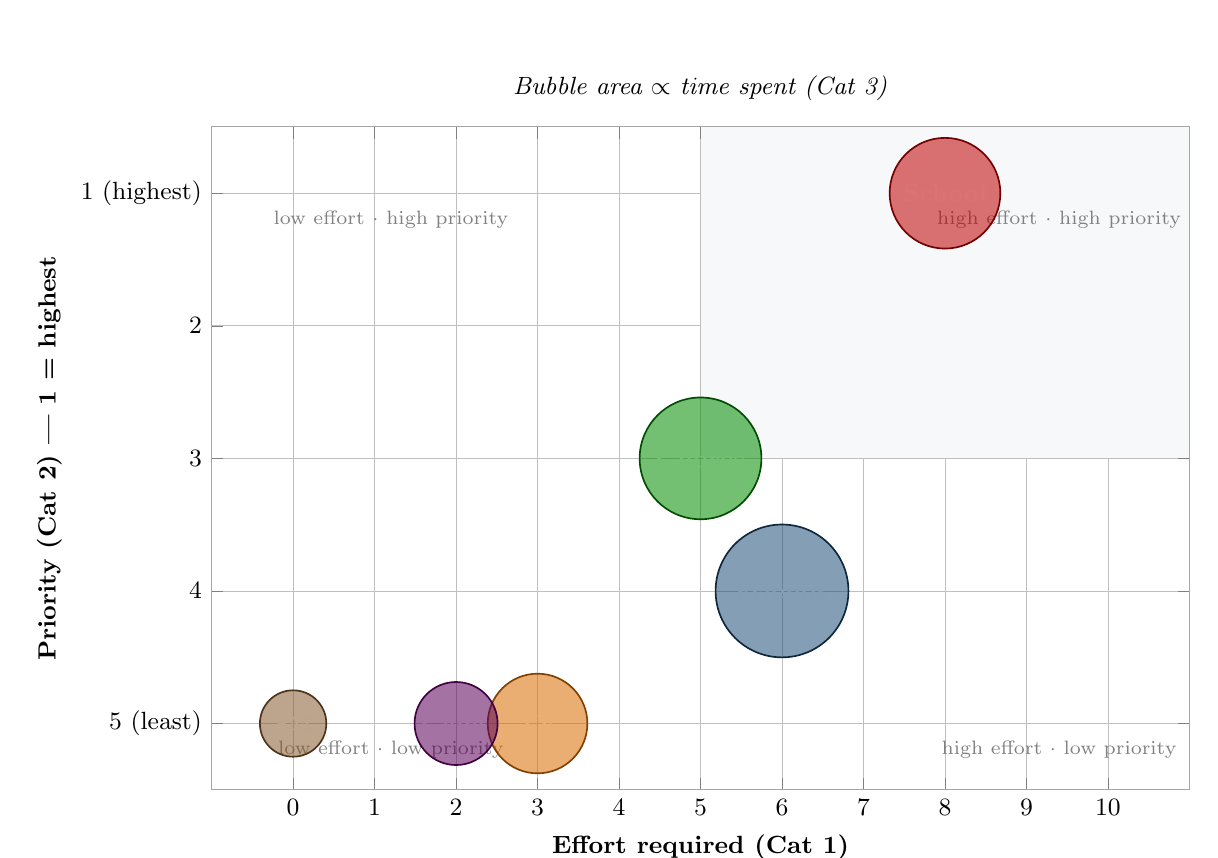
\begin{tikzpicture}
\begin{axis}[
    width=14cm, height=10cm,
    xlabel={\textbf{Effort required (Cat 1)}},
    ylabel={\textbf{Priority (Cat 2) --- 1 = highest}},
    xmin=-1, xmax=11,
    ymin=0.5, ymax=5.5,
    y dir=reverse,
    xtick={0,1,2,3,4,5,6,7,8,9,10},
    ytick={1,2,3,4,5},
    yticklabels={1 (highest),2,3,4,5 (least)},
    grid=both,
    grid style={line width=0.2pt, draw=gray!30},
    major grid style={line width=0.3pt, draw=gray!50},
    axis line style={draw=gray!70},
    tick label style={font=\small},
    label style={font=\small},
    title={\small\textit{Bubble area $\propto$ time spent (Cat 3)}},
]

% Quadrant guide shading
\fill[accent!4] (axis cs:5,0.5) rectangle (axis cs:11,3);

% Each scatter mark: position on (effort,priority); mark size scaled by sqrt(time)
% mark size = 6 + 6*sqrt(time)  -> visually proportional to area
\addplot[only marks, mark=*, mark options={fill=accent2,draw=accent2!60!black,fill opacity=0.55,line width=0.6pt}, mark size=20] coordinates {(8,1)};
\node[font=\small\bfseries, white] at (axis cs:8,1) {School};

\addplot[only marks, mark=*, mark options={fill=accent,draw=accent!50!black,fill opacity=0.55,line width=0.6pt}, mark size=24] coordinates {(6,4)};
\node[font=\small\bfseries, white] at (axis cs:6,4) {Friends};

\addplot[only marks, mark=*, mark options={fill=green!55!black,draw=green!30!black,fill opacity=0.55,line width=0.6pt}, mark size=22] coordinates {(5,3)};
\node[font=\small\bfseries, white] at (axis cs:5,3) {Chores};

\addplot[only marks, mark=*, mark options={fill=orange!85!black,draw=orange!50!black,fill opacity=0.55,line width=0.6pt}, mark size=18] coordinates {(3,5)};
\node[font=\footnotesize\bfseries, white] at (axis cs:3,5) {TV};

\addplot[only marks, mark=*, mark options={fill=violet!70!black,draw=violet!50!black,fill opacity=0.55,line width=0.6pt}, mark size=15] coordinates {(2,5)};
\node[font=\footnotesize\bfseries, white] at (axis cs:2,5) {Game};

\addplot[only marks, mark=*, mark options={fill=brown!70!black,draw=brown!40!black,fill opacity=0.55,line width=0.6pt}, mark size=12] coordinates {(0,5)};
\node[font=\scriptsize\bfseries, white] at (axis cs:0,5) {SM};

% Quadrant labels
\node[font=\scriptsize, gray] at (axis cs:9.4,1.2) {high effort $\cdot$ high priority};
\node[font=\scriptsize, gray] at (axis cs:9.4,5.2) {high effort $\cdot$ low priority};
\node[font=\scriptsize, gray] at (axis cs:1.2,1.2) {low effort $\cdot$ high priority};
\node[font=\scriptsize, gray] at (axis cs:1.2,5.2) {low effort $\cdot$ low priority};

\end{axis}
\end{tikzpicture}
\caption{Workload-pressure scatter. The plot reveals a structural inversion: the largest bubble (\textbf{Friends}, time = 7) sits at priority 4, while the highest-priority activity (\textbf{School}, priority 1, effort 8) is represented by a smaller bubble (time = 5). Activities clustered along the bottom row at priority~5 collectively consume more time than School and Chores combined.}
\label{fig:scatter}
\end{figure}

\subsection{Reading the overlap pattern}
The visual reveals three diagnostic patterns:
\begin{enumerate}[leftmargin=1.6em, itemsep=2pt]
  \item \textbf{Inverted gradient.} Bubble size should \emph{decrease} as priority number increases (top to bottom). The actual pattern shows the opposite trend from priority 1 $\rightarrow$ 4, only correcting at priority 5.
  \item \textbf{Largest bubble in low-priority territory.} \textbf{Friends} (priority 4) is the largest bubble on the chart --- a textbook misallocation signature.
  \item \textbf{Effort/time mismatch on the priority-1 item.} \textbf{School} sits in the upper-right corner (high effort, high priority) but is allocated less time than three lower-priority activities combined.
\end{enumerate}

% =====================================================================
\section{Quantitative Analysis}
\label{sec:analysis}

\subsection{Time-share decomposition}
With a total time budget of 27 normalized units, the share allocated to each category is:

\begin{table}[h]
\centering
\renewcommand{\arraystretch}{1.2}
\begin{tabular}{lcccl}
\toprule
\textbf{Category} & \textbf{Priority} & \textbf{Time} & \textbf{Share} & \textbf{Alignment} \\
\midrule
School        & 1 & 5 & 18.5\,\% & \textcolor{accent2}{\textbf{Under-allocated}} \\
Chores        & 3 & 6 & 22.2\,\% & Reasonable \\
Friends       & 4 & 7 & \textbf{25.9\,\%} & \textcolor{accent2}{\textbf{Over-allocated}} \\
TV            & 5 & 4 & 14.8\,\% & Over-allocated \\
Video Game    & 5 & 3 & 11.1\,\% & Mild over \\
Social Media  & 5 & 2 & ~7.4\,\% & Tolerable \\
\midrule
\multicolumn{2}{l}{\textit{Low-priority total} (priority $\geq 4$)} & \textbf{16} & \textbf{59.3\,\%} & --- \\
\bottomrule
\end{tabular}
\caption{Time-share decomposition by priority tier.}
\label{tab:share}
\end{table}

\subsection{Pressure justification check}
The reported pressure of $P_\text{felt} = 8$ exceeds the baseline $P_\text{base} = 5$ by $\Delta P = +3$. Three independent indicators support the pressure as mechanically justified rather than spurious:

\begin{enumerate}[leftmargin=1.6em, itemsep=2pt]
  \item \textbf{Effort/time deficit.} School requires effort = 8 to produce desired outcomes but is allocated only time = 5. The pressure signal correctly prices this gap.
  \item \textbf{Inverted time-priority gradient} (see Section~\ref{sec:chart}, point 1).
  \item \textbf{Friends-as-largest-bubble distortion.} A 1.40$\times$ time excess over the priority-1 item, three priority tiers lower.
\end{enumerate}

\begin{keybox}[Justification ruling]
The pressure would be \emph{unjustified} only if School were already receiving the largest time slice. It is not. Therefore $P_\text{felt} = 8$ is a correctly calibrated stress signal, and reducing it requires \textbf{structural reallocation, not stress-management techniques}.
\end{keybox}

% =====================================================================
\section{Corrective Measures}
\label{sec:fixes}

Recommended actions, ranked by leverage:

\begin{enumerate}[leftmargin=1.6em, itemsep=4pt]
  \item \textbf{Rebalance Friends time: 7 $\rightarrow$ 4--5.}\\
        Reclaims $\sim$2--3 time units from the largest single misallocation.
  \item \textbf{Reallocate to School: 5 $\rightarrow$ 7--8.}\\
        Brings time into alignment with the effort = 8 demand. Pressure should regress toward baseline within $\sim$1--2 weeks of sustained reallocation.
  \item \textbf{Cap TV at 2--3.}\\
        Priority-5 items should not approach School in time-share.
  \item \textbf{Leave Chores unchanged.}\\
        Priority 3 / time 6 / effort 5 is the only category with proportionate allocation.
  \item \textbf{Do not target Social Media or Video Games.}\\
        Combined they account for only 5 time units (18.5\,\%); cutting them is low-yield and removes useful decompression valves.
\end{enumerate}

% =====================================================================
\section{Criticality Scoring}
\label{sec:criticality}

Each category is scored 0--10 on its criticality \emph{relative to the central question} (whether the felt pressure is justified, and what to change).

\begin{table}[h]
\centering
\renewcommand{\arraystretch}{1.25}
\begin{tabular}{l c >{\raggedright\arraybackslash}p{8.5cm}}
\toprule
\textbf{Category} & \textbf{Criticality} & \textbf{Rationale} \\
\midrule
Friends time allocation & \textcolor{accent2}{\textbf{9 / 10}} & Largest single misallocation; biggest bubble at low priority. Highest-leverage fix in the system. \\
School time allocation  & \textcolor{accent2}{\textbf{9 / 10}} & Same issue, receiving side. Every reclaimed unit must land here to close the effort/time gap. \\
TV time                 & 5 / 10 & Secondary trim; meaningful but not pivotal. \\
Chores                  & 2 / 10 & Roughly correct, leave alone. \\
Video Game              & 2 / 10 & Not worth restructuring. \\
Social Media            & 1 / 10 & Already minimal. \\
\bottomrule
\end{tabular}
\caption{Criticality ranking with respect to closing the pressure gap.}
\label{tab:crit}
\end{table}

% =====================================================================
\section{Conclusion}

The 8/10 pressure reading is functioning as a correctly calibrated alarm, not noise. The fix is not to work harder on the priority-1 item, but to \textbf{transfer 2--3 time units out of Friends (and 1 out of TV) into School}. Closing the structural input/output gap should regress the pressure toward the 5/10 homeostatic baseline without requiring any change in productivity, discipline, or coping strategy.

\begin{keybox}[Single most actionable change]
Move 2--3 time units per week from \textbf{Friends} into \textbf{School}. Hold for 14 days. Re-rate pressure. If $P_\text{felt} \leq 6$, the diagnosis is confirmed. If not, escalate to a finer-grained re-measurement.
\end{keybox}

\vspace{1em}
\hrule height 0.4pt
\vspace{0.4em}
{\small\color{rule}\textit{This report is a structured analytical aid based on coarse-grained self-report. It does not constitute medical, psychological, or clinical advice. All numeric claims have been recomputed from the input data; all coordinates in Figure~\ref{fig:scatter} are derived from the data table without manual placement adjustment.}}

\end{document}
